\resourceheading{7}{Day Recap Evidence Story}{Collective memory, responsive planning, and multi-audience communication\par}{Students, teachers, families, collaborators, and program leaders}{Five implemented and reviewed EDU486 day-recap presentations}

\vspace{-0.5cm}
\toolsection{The Existing Camp Artifact}

A communication route matters beyond the moment only if the learner's meaning survives in the shared record. The camp team completed one reviewed recap presentation for each documented camp day, Days 1--5. Each deck reconstructed the day's activity sequence, connected youth actions and words to the shared scientific model, preserved evidence limits, and made the next question visible. The recap created a shared memory that youth could revisit, helped instructors decide what should continue or change, and gave collaborators and families a defensible account of what happened \citep{campEvidence2026}. This is communication and positive behavioral support because it resists adult shorthand such as ``engaged'' or ``off task.'' Instead, the recap preserves what learners did, what evidence they worked with, what questions remained, and how participation changed. A learner can point, tell, show, partner, pass, and return while the rigorous group story remains available. Communication becomes reliable when student contributions can revise the shared account and influence what happens next \citep{peckhamhardin2015behavior}.

\toolsection{The Completed Day Recap}

\begin{center}
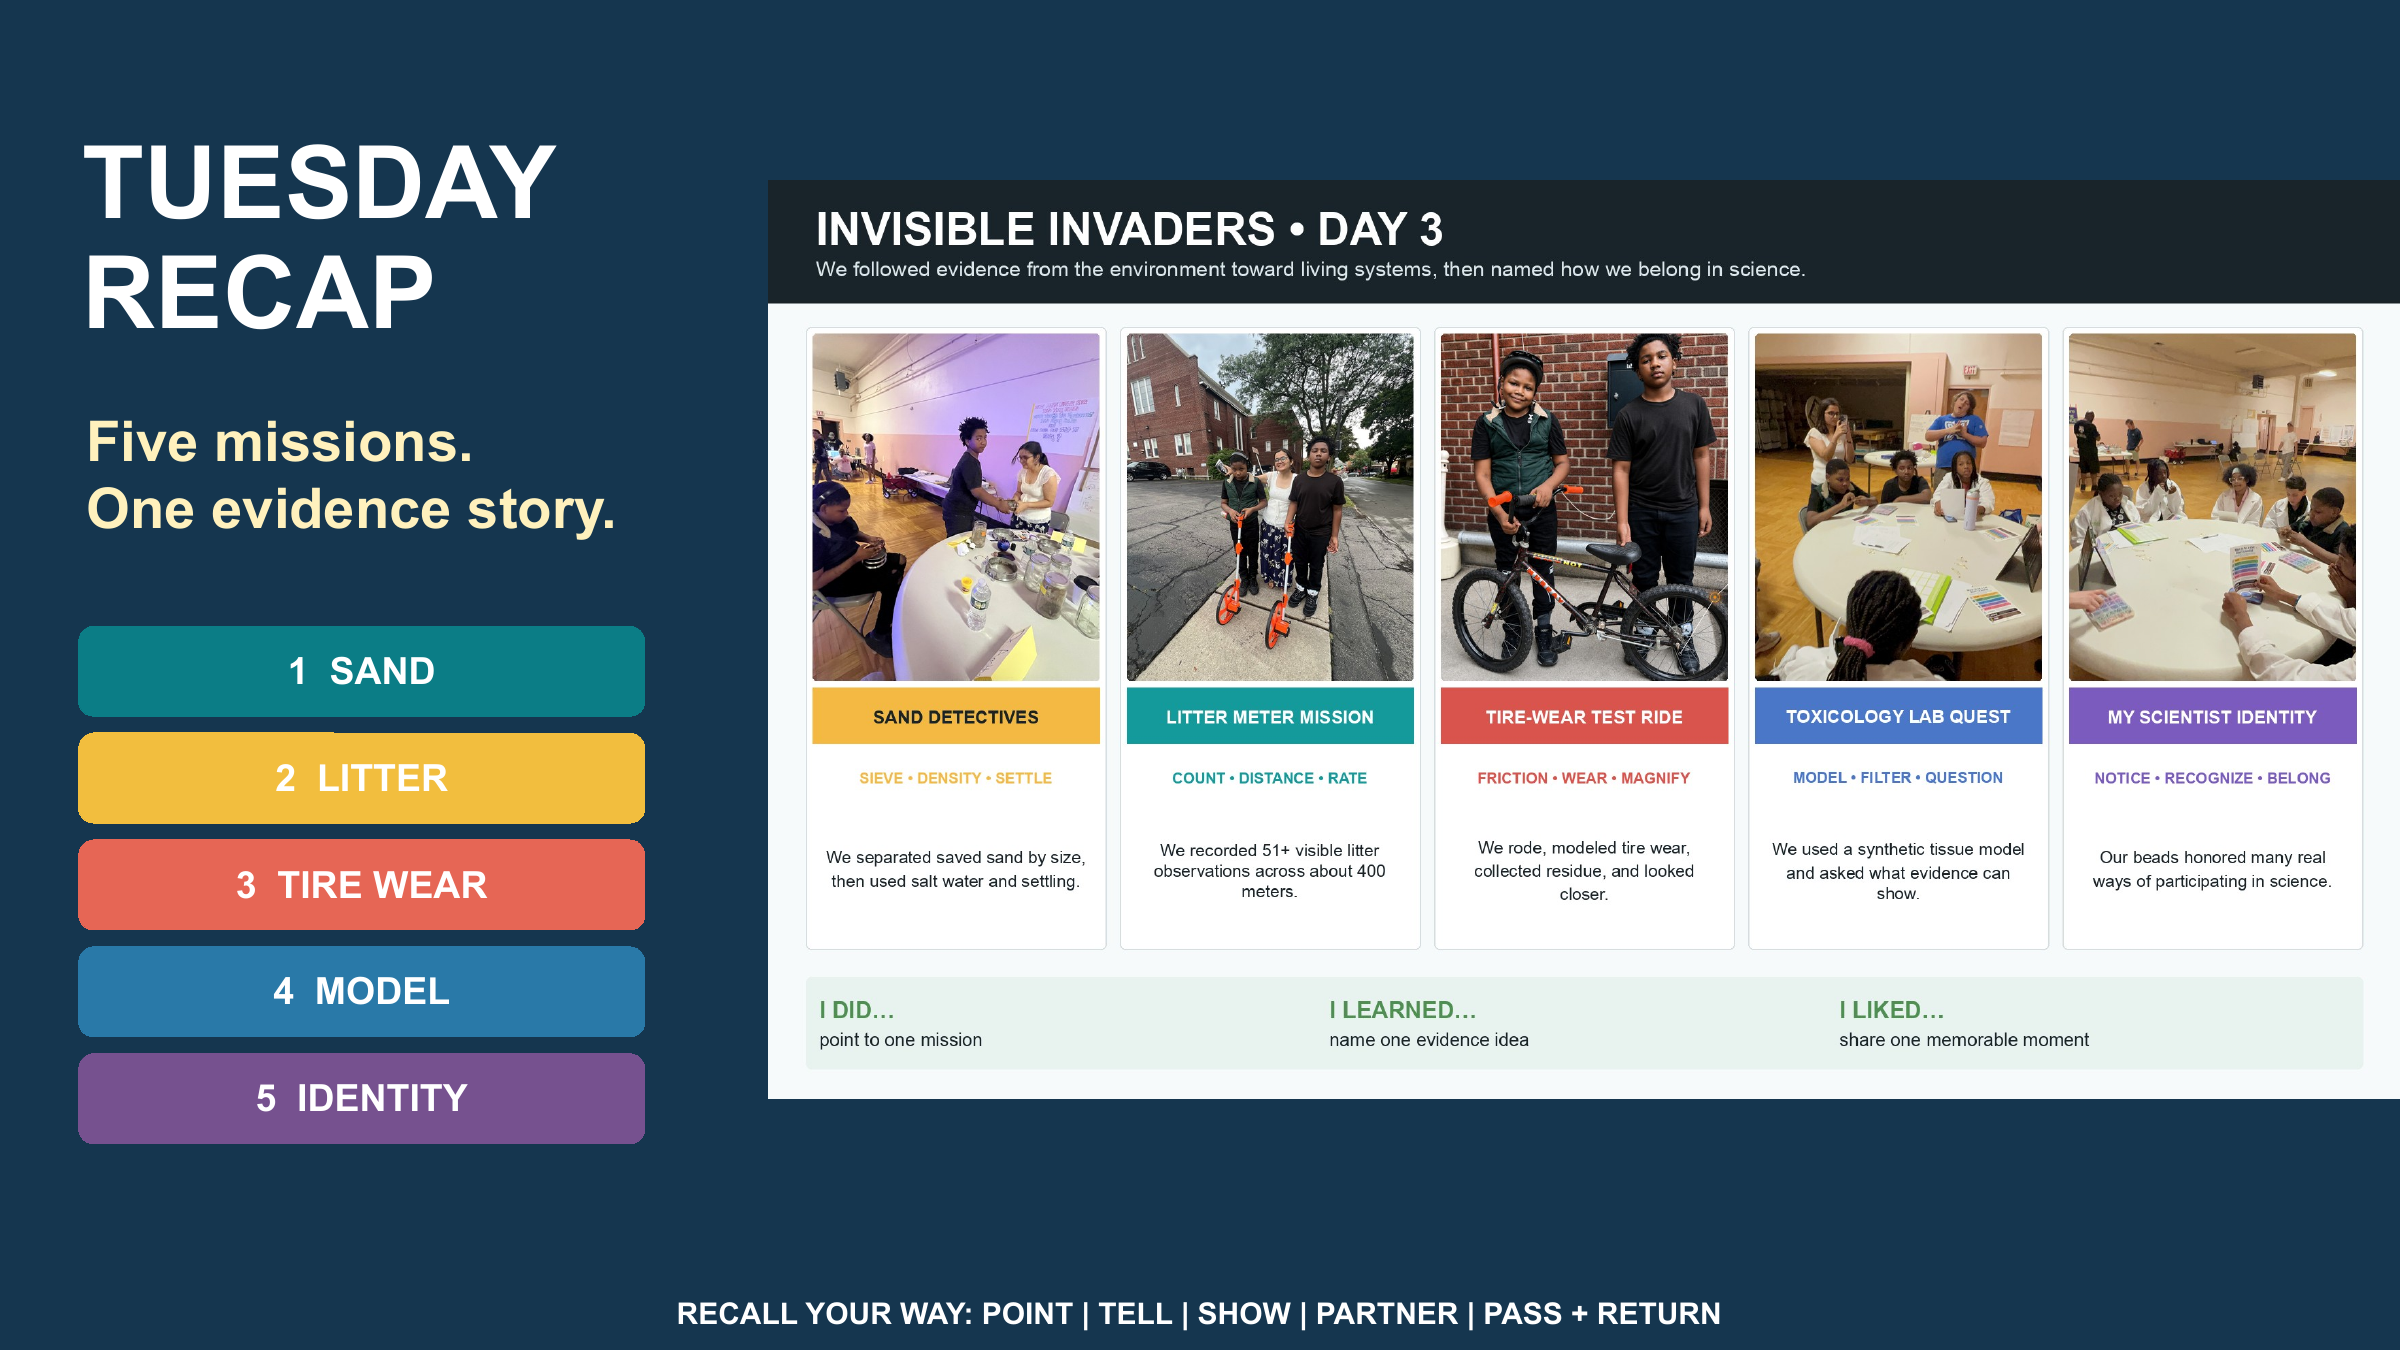
\includegraphics[
  width=0.85\textwidth,
  keepaspectratio
]{assets/artifact-previews/day-recap-day3-example.png}

% \vspace{0.015in}
\parbox{0.94\textwidth}{\centering
\textbf{\color{DeepNavy}Public-safe Day 3 recap example.}
The recap reconstructs a shared investigation through \textit{mix, filter, and compare}, reconnects the activity to the scientific model, preserves an explicit evidence limit, and keeps multiple recall routes available. The same record supports student memory, partner conversation, family communication, and planning for what should happen next.}

% \vspace{0.04in}
\makebox[\textwidth][c]{%
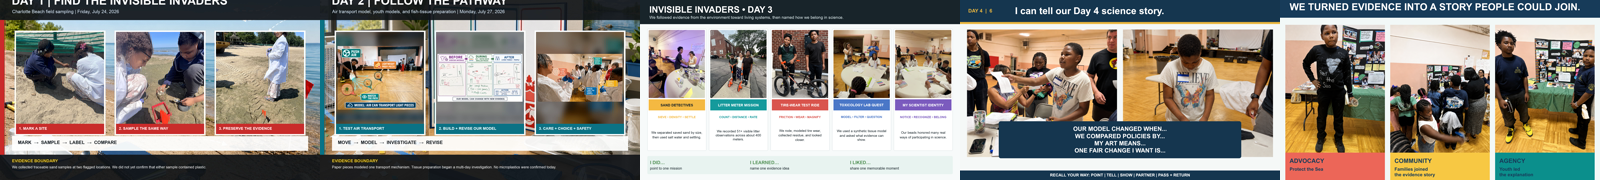
\includegraphics[
  width=1.0\textwidth,
  trim=0 100 0 100,
  clip
]{assets/artifact-previews/five-day-recap-strip.png}%
}
% \vspace{0.01in}
\parbox{0.94\textwidth}{\centering\textbf{Days 1--5 archive:}
locate the problem; collect and compare evidence; revise the model; examine living systems; and carry evidence into youth-led community action.}

\end{center}

\newpage
% \small

\toolsection{Build the Recap Before Planning Tomorrow}
\begin{spacing}{1.0}
\begin{enumerate}
  \item \textbf{Inventory what actually happened.} Record every activity, including what changed order, shortened, moved, expanded, or did not happen.
  \item \textbf{Triangulate the evidence.} Use artifacts, photographs, video/transcript records, student memos, measurements, and instructor notes according to what each source can actually establish.
  \item \textbf{Preserve youth meaning.} Record direct words, questions, choices, dislikes, model revisions, and contributions; do not infer understanding, emotion, or motivation from appearance alone.
  \item \textbf{Rebuild the shared storyline.} Show what the group did, what evidence changed the explanation, what remained uncertain, and what question should continue.
  \item \textbf{Keep communication and re-entry visible.} Preserve routes such as point, tell, show, partner, pass, and return, along with role changes, movement, sensory boundaries, and later re-entry.
  \item \textbf{Close the loop.} Use the reviewed recap to decide what to keep, change, stop, or investigate next, then circulate only the version appropriate for each approved audience.
\end{enumerate}
\end{spacing}

\toolsection{One Story, Four Feedback Loops}

\renewcommand{\arraystretch}{1.08}
\setlength{\tabcolsep}{4pt}

\begin{tabularx}{\textwidth}{
>{\bfseries\RaggedRight\arraybackslash}p{0.70in}
>{\RaggedRight\arraybackslash}p{2.98in}
>{\RaggedRight\arraybackslash}X}

\rowcolor{MidTeal}
\color{white}Audience &
\color{white}What the Recap Returns &
\color{white}What It Can Change \\

Youth &
A visible memory of the activities, their work, model changes, choices, and questions &
Correction, ownership, re-entry, reflection, and the next investigation \\

\rowcolor{SoftGray}
Teaching team &
One reviewed evidence story instead of isolated impressions or behavior labels &
Pacing, materials, questions, roles, supports, participation routes, and what stops/continues \\

Program partners &
Traceable claims, participation routes, plan decisions, revisions, and evidence limits &
Institutional understanding, resource decisions, and accountability for adult design \\

\rowcolor{SoftGray}
Families &
Concrete account of what youth did, shared, asked, learned, disliked, or wanted &
Family conversation, continuity across settings, and knowledge that can return to teachers\\

\end{tabularx}

\toolsection{Evidence That Changed the Story \& Puzzle Plan and EQUITAS in Practice}

The recaps changed how camp events were interpreted. Day 2 records the racket game as a movement reset and relationship route. Day 3 keeps ``point, tell, show, partner, pass + return'' available across the recap so remembering the day does not depend on one communication mode. The later youth retrospective asks for less rushing, more investigation time, more physical activity, a non-fish route to the same scientific idea, and numbered showcase stations. The evidence therefore changes the shared story and the design of what should happen next \citep{campEvidence2026}. The Puzzle Plan brings student voice together with artifacts, context, scientific evidence, and adult decisions. EQUITAS asks whose words enter the recap, who appears only as a body, and who gets to correct the institutional story. A recap becomes access-to-agency only when youth work can alter the record, interpretation, lesson, understanding, or what families receive.

\reflectionbox{\textbf{Artifact proof:} Five reviewed recap decks for Days 1--5 collectively preserve activities, youth contributions, communication routes, evidence limits, model revisions, and next questions. Day 6 has a clean retrospective transcript. Day 5 has photographs and a same-session transcript; its recap explicitly limits what photographs can establish \citep{campEvidence2026}.}

\adaptationbox{A recap can still privilege the most verbal, photographed, or adult-approved account. Invite correction through speech, AAC, writing, drawing, pointing, shared visuals, home language, partner support, or private review. Preserve disagreement, refusal, uncertainty, and ``not yet.''}

% \sourcebox{\scriptsize Camp recap archive \citep{campEvidence2026}; communication and behavior \citep{peckhamhardin2015behavior}.}

\normalsize